\chapter{Bipartite Perfect Matching}
\section{A \textsc{RNC} Algorithm for \textsc{Search-PM}}\label{rnc-bipartite-pm}
We will recall the \textsc{RNC} algorithm of Mulmuley, Vazirani and Vazirani \cite{MulmuleyVaziraniVazirani_1987_Mia_CONF} for the construction of a perfect matching (\textsc{Search-PM}). Though the algorithm works for any graph, we will only consider the bipartite graphs here.

Let $G=(V,E)$ be a bipartite graph with vertex partitions $L=\{u_1,\dots, u_{\frac{n}{2}}\}$ and $R=\{v_1,\dots, v_{\frac{n}2}\}$ and a weight function $w$. Consider the following $\frac{n}2\times \frac{n}{2}$ matrix $A$ associated with $G$, \[
	A(i,j)=\begin{cases}
		2^{w(e)} & \text{if $e=(u_i,u_j)\in E$} \\
		0        & \text{otherwise}
	\end{cases}
\]
The algorithm then computes the determinant of $A$. Now \begin{align*}
	\det(A) & = \sum\limits_{\pi\in S_{\frac{n }{2}}}^{} sgn(\pi)\prod_{i=1}^{\frac{n }{2}} A(i,\pi(i)) \\ & = \sum\limits_{M:\text{PM in $G$}}^{}sgn(M)2^{w(M)}
\end{align*}
The second equation holds since the product $\prod\limits_{i=1}^{\frac{n}2} A(i,\pi(i))$ is nonzero if and only if the permuation $\pi$ corresponds to a perfect matching. Here $sgn(M)$ is the sign of the corresponding permutation.

If the graph $G$ does not have a perfect matching then we have $\det(A)=0$. However if the graph $G$ has perfect matchings, $\det(A)$ maight equal to 0 due to cancellation due to $sgn(M)$. To avoid such cancellations, one needs to design the weight function $w$ cleverly. In particular if $G$ has a perfect matching and $w$ is isolating then the  minimum weight perfect matching can not be canceled with other terms as there is unique minimum weight perfect matching.

Given an isolating weight assignment for $G$, one can construct the minimum weight perfect matching in \textsc{NC}. Let $M^*$ be the unique minimum weight perfect matching in $G$ w.r.t $w$. First we find $w(M^*)$ be finding out the highest power of $2$ that divides $\det(A)$ since  after $2^{w(M^*)}$ will not divide the monomial corresponding to $M^*$ and that monomial survives in $\det(A)$. So more that after $2^{w(M^*)}$ it will not divide $\det(A)$. Now choose an $(u_i,u_j)=e\in E$ then compute the determinant of the minor $A_{i,j}$ which is basically associated with $G-e$. If the highest power of 2 that divides $\det(A_{i,j})$ is larger than the $2^{w(M^*)}$ then $e\in M^*$. Doing this in parallel for each edge, we can find all the edges in $M^*$.

By \thrmref{th:isolation-lemma}	we have an isolating weight with high probability. Moreover the weights chosen by the isolation lemma are polynomially bounded. Therefore the entries of in matrix $A$ have polynomially many bits. Hence it suffices to compute the determinant in $\textsc{NC}^2$ \cite{Berkowitz_1984_Oct}. Also the construction is in $\textsc{NC}^2$. There fore this yields an $\textsc{RNC}$-algorithm for $\textsc{Search-PM}$.

\section{A \textsc{Quasi-NC} Algorithm using Isolation}\label{quasinc-bipartite-pm}
Let $G=(V,E)$ be given bipartite graph. In the following discussion we will assume that $G$ has perfect matchings. Our goal is to isolate one of the perfect matchings in $G$ by any appropriate weight function. We will also show that if $G$ does not have any perfect matchings then our algorithm will detect this. In the following discussion we will prove this theorem
\begin{Theorem}{\cite[Theorem 3.1]{FennerGurjarThierauf_2016_Bpm_CONF}}{pm-searchpm-in-quasinc}
	For bipartite graphs, \textsc{PM} and \textsc{Search-PM} are in $\textsc{Quasi-NC}^2$
\end{Theorem}

We will construct an isolating weight function for bipartite graphs. The idea is to create a weight function which ensures nonzero circulations for a small set of cycles in a black-box way i.e. without having being able to compute the set efficiently. Then we will show that if we construct a smaller graph wrt this weight function then we don't have those small cycles with nonzero circulations then we have the number of cycles with twice the size of the previous ones are polynomially bounded. Then we proceed to create a new weight function which will give nonzero circulations to all the cycles with twice the size. And this way we will continue. This same type of idea we will repeatedly use with necessary modifications in \autoref{linear-matroid-intersection} and \autoref{fractional-matroid-matching}.

The idea above to create a weight function which gives nonzero circulation to every nice cycles in $G$ actually works because  then we have unique perfect matching by \lemref{th:all-nice-cycles-nonzero-circulation-unique-perfect-matching}
\subsection{Isolating Small Cycles}

The following lemma describes a standard trick to create a weight function for a small set of cycles in graph.
\begin{lemma}{\cite{ChariRohatgiSrinivasan_1993_Rou_CONF}}{weight-for-all-s-cycles-to-have-nonzero-circulations}
	Let $G$ be a graph with $n$ vertices. Then for any number $s$, one can construct a set of $O(n^2s)$ weight assignments with weights bounded by $O(n^2s)$, such that for any set of $s$ cycles, one of the weight assignments gives nonzero circulation to each of the $s$ cycles.
\end{lemma}
\begin{proof}
	Let us first assign exponentially large weights. Let $e_1, e_2,\dots , e_m$ be some enumeration of the edges of $G$. Define  a weight function $w$ by $w(e_i)=2^{i-1}$ for $i\in [m]$. Then clearly every cycle has a nonzero circulation. However we want to achieve this with small weights.

	We consider the weight assignment modulo small numbers i.e. the weight function is $\{w\bmod j\mid 2\leq j\leq t\}$ for some appropriately chosen $t$. We want to show that for any fixed set of $s$ cycles $\{C_1,\dots, C_s\}$ one of these assignments will work when $t$ is chosen large enough.

	Now we want $$\exs\ j\leq t,\ \forall\ i\leq s,\ c_w(S_i)\neq 0\iff \exs\ j\leq t,\ \prod_{i=1}^s c_w(C_i)\neq 0\bmod j$$In other words we want $$lcm(2,3,\dots, t)\nmid \prod_{i=1}^t c_w(C_i)$$Hence if we take $t$ such that $lcm(2,3,\dots, t)> \prod\limits_{i=1}^t c_w(C_i)$ then we are done.

	Now the product $\prod\limits_{i=1}^t c_w(C_i)$ is bounded by $2^{n^2s}$. This is because with exponential weights {like in the RNC algorithm} of \autoref{rnc-bipartite-pm} we have an isolating perfect matching so we need weights less than that and therefore the new weights are bounded by the exponential weights for which weight of a cycle can at most be $2^{n^2}$ and since there are $s$ many cycle we have the bound $2^{n^2s}$. So if we have $t$ such that $lcm(2,3,\dots, t)>2^{n^2s}$ then we are done. Now $lcm(2,3,\dots,t)>2^t$ for $t\geq 7$. Thus choosing $t=n^2s$ suffices. Clearly the weights are bounded by $t=n^2s$.
\end{proof}

\subsection{Union of Minimum Weight Perfect Matchings}
Let us assign a weight function for bipartite graph $G$ which gives nonzero circulations to all small cycles. Consider a new graph $G_1$ which obtained by the union of minimum weight perfect matchings in $G$. Out hope is that $G_1$ is significantly smaller than $G$.
\nt{We don't know if $G_1$ can be efficiently created from $G$ as determinant of the bi-adjacency matrix with weights in the {like in the RNC algorithm} of \autoref{rnc-bipartite-pm} be zero and therefore we can not use that way to obtain perfect matchings. We will show we don't need to construct $G_1$. It is just used n the argument. Our final weight assignment will be completely black-box}

We will also show by the following lemma that why this technique only works for biparitte graphs, not in general graphs i.e. $G_1$ constructed from minimum weight perfect matchings in $G$ contains no other prefect matching than these. For general graph this does not hold:

\begin{center}
	\begin{minipage}{0.3\textwidth}
		\begin{center}
			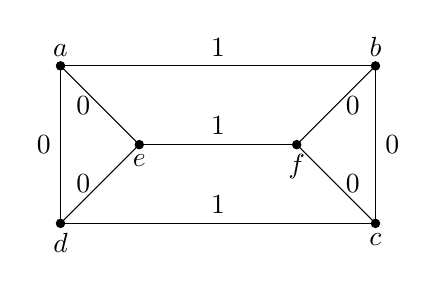
\begin{tikzpicture}
				\draw (-2,1) node[above]{$a$} -- node[midway,above] {1} (2,1)node[above]{$b$} --node[midway,right]{0}  (2,-1)node[below]{$c$} --node[midway,above]{1} (-2,-1)node[below]{$d$} --node[midway,left]{0} cycle;
				\draw (-2,1) --node[midway,left]{0} (-1,0) --node[midway,left]{0} (-2,-1);
				\draw (2,1) --node[midway,right]{0} (1,0) --node[midway,right]{0} (2,-1);
				\draw (1,0)node[below]{$f$} --node[midway,above]{1}  (-1,0)node[below]{$e$};
				\filldraw (-2,1) circle (1.5pt);
				\filldraw (-2,-1) circle (1.5pt);
				\filldraw (2,-1) circle (1.5pt);
				\filldraw (2,1) circle (1.5pt);
				\filldraw (1,0) circle (1.5pt);
				\filldraw (-1,0) circle (1.5pt);
			\end{tikzpicture}
		\end{center}
	\end{minipage}\hspace{1cm}
	\begin{minipage}{0.6\textwidth}
		In this graph we will denote the edge connected vertices $a,b$ to be $e_{ab}$. And this way we will denote all the edges. Then the minimum weight perfect matchings have weight 1 and they are $$\{e_{ad},e_{bc},e_{ef}\}, \quad \{e_{ac}, e_{bf}, e_{cd}\},\quad \{e_{de}, e_{cf}, e_{ab}\}$$Then their union has the perfect matching $\{e_{ab},e_{cd},e_{ef}\}$ which has weight 3 and not a minimum weight perfect matching.
	\end{minipage}
\end{center}

The fact that $G_1$ has only minimum weight perfect matching is equivalent to saying that every nice cycle has zero circulation. The following lemma proves even stronger statement that every cycles has zero circulation (not necessarily nice cycles.)
\begin{Lemma}{\cite[Lemma 3.2]{FennerGurjarThierauf_2016_Bpm_CONF}}{nozero-circulation-notin-minimum-weight-perfect-matching-graph}
	Let $G=(V,E)$ be a bipartite graph with weight function $w$. et $C$ be a cycle in $G$ such that $c_w(C)\neq 0$. Let $E_1$ be the union of all minimum weight perfect matchings in $G$. Then the graph $G_1=(V,E_1)$ does not contain $C$.
\end{Lemma}
\begin{proof}
	Consider the perfect matching polytope of $G$, $PM(G)$. Let the weight of the minimum weight perfect matching in $G$ be $q$. Let $x_1,x_2,\dots,x_t$ be all the minimum weight perfect matching points of $G$ i.e. corners of $PM(G)$ corresponding to weight $q$. Consider the average point $x\in PM(G)$ of these perfect matching points, $x=\frac{x_1+x_2+\cdots+x_t}{t}$. Clearly we have $w(x)=q$. And since each edge of $G_1$ participates in a minimum weight perfect matching for $x=(x_e)_{e\in E}$ we have $x_e\neq 0$ $\forall\ e\in E$.

	Now consider a cycle $C$ with $c_w(C)\neq 0$. Suppose $C=(e_1,e_2,\dots, e_{k})$ and all the edges of $C$ are in $E_1$. We will show that if we move from point $x$ along the cycle $C$ we reach a point in $PM(G)$ with a weight smaller than $q$.

	Consider the point $y$ defined as $$\forall\ e\in E,\quad y_e=\begin{cases}
			x_e+(-1)^i\eps\& \text{if $e=e_i$ for some $i\in[k]$} \\
			x_e & \text{o/w}
		\end{cases}$$for some $\eps\neq 0$. Clearly $x-y$ has nonzero coordinates only on the edges of the cycle $C$, by alternating between $\eps$ and $-\eps$. Hence $$w(x)-w(y)=w(x-y)=\pm c_w(C)\neq 0$$

	Now we take $\eps$ in the following way:
	\begin{itemize}
		\item Take $sgn(\eps)$ such that $w(x-y)>0$.
		\item Take $\eps$ small enough such that $y_e\geq 0\ \forall\ e\in E$.
	\end{itemize}

	After choosing such $\eps$ since $w(x)-w(y)=w(x-y)>0$ we have $q=w(x)>w(y)$. Now we will show that $y\in PM(G)$. To show that we will sow that $y$ fulfills the conditions of \thrmref{th:bipartite-polytope-equations}. Now the second condition that $y_e\geq 0$ for all $e\in E$ is already satisfied by the choice of $\eps$. So we only need to show that for any $v\in V$ $$\sum_{e\in \delta(v)}y_e=1$$To show this we consider 2 cases:
	\begin{enumerate}[label=\bfseries Case \arabic*:,leftmargin=1.7cm]
		\item $v\notin C$. Then $\forall \ e\in \dl(v)$ we have $e\notin C$. So $y_e=x_e$. Since $x\in PM(G)$ we have $$\sum_{e\in\dl(v)}x_e=1\implies \sum_{e\in \dl(v)}y_e=1$$
		\item $v\in C$. Let $e_j$ and $e_{j+1}$ are the edges incident on $v$ in $C$. Then $$y_{e_j}=x_{e_j}+(-1)^{j}\eps\qquad \text{and}\qquad y_{e_{j+1}}=x_{e_{j+1}}+(-1)^{j+1}\eps\qquad \forall\ e\in \dl(v)-\{e_{j},e_{j+1}\},\ y_e=x_e$$So\begin{align*}
			      \sum_{e\in \dl(v)}y_e & = \lt[\sum_{e\in \dl(v)-\{e_j,e_{j+1}\}}x_e\rt]+\lt[x_{e_j}+(-1)^j\eps\rt]+\lt[x_{e_{j+1}}+(-1)^{j+1}\eps\rt] \\
			                            & = \lt[\sum_{e\in \dl(v)}x_e\rt]+(-1)^j\eps+(-1)^{j+1}\eps = \sum_{e\in \dl(v)}x_e=1
		      \end{align*}
	\end{enumerate}
	So the point $y$ satisfies the property $\sum\limits_{e\in\dl(v)}=1$ forall $v\in V$. Hence $y\in PM(G)$. Now since $w(y)<q$ there must be a corner point of the polytope which corresponds to a perfect matching in $G$ with weight less than $q$. This contradicts the minimality of $q$. Hence $C$ is not in $G_1$.
\end{proof}
This technique of moving along the cycle has been used by Mahajan and Varadarajan in \cite{MahajanVaradarajan_2000_AnN_CONF}. Now We will show another proof of this lemma by Rao, Shpilka  and Wigderson in \cite{GoldwasserGrossman_2017_BPM}.\vspace*{\baselineskip}


\begin{alternate-proof}[{\cite[Proof of Lemma 6]{GoldwasserGrossman_2017_BPM}}]
Let $G'$ be the multigraph obtained by taking disjoint union of all minimum weight perfect matchings (i.e. if an edge appears in $k$ many minimum weight perfect matchings of $G$ then $G'$ contains  $k$ copies of the edge.
\nt{$G'$ is a regular graph since it is a disjoint union of matchings and matchings are regular graph of degree 1.}


Suppose there exists a cycle $C$ of non zero circulation in $G_1$. Since the cycle is in $G_1$ then this cycle is also in $G'$. WLOG  assume that the sum of the weights of the odd edges of $C$ is larger than the sum of the weights of the even edges. Then we can remove a single copy of each odd edges of $C$ from $G'$ and add a single copy of each even edges of $C$ to $G'$ and we call this new graph $G''$

Suppose $q$ be the minimum weight of a matching in $G$. Suppose $G$ has $d$ minimum weight matchings. Then sum of the weights of the edges in $G'$ is $qd$.	However, the total weight of all edges in in $G''$ is lower than the total weight of all edges in $G'$. We know  that $G''$ is a regular bipartite graph of degree $d$ and therefore by \lemref{th:regular-bipartite-graph-union-pm} it is an union of $d$ perfect matchings.

If we decompose $G''$ into $d$ perfect matchings, it is impossible that they all have weight at least $q$ as $G''$ has total weight less than $qd$. Therefore $G''$ has a matching of weight less than $q$, which contradicts the minimality of $q$.
\end{alternate-proof}
A consequence of this lemma is that $G_1$ has no other perfect matchings than the ones used to define $G_1$ cause if $M_0$ and $M_1$ be two different perfect matchings in $G_1$ then $M_0\triangle M_1$ forms a set of nice cycles and by the \lemref{th:nozero-circulation-notin-minimum-weight-perfect-matching-graph} the circulations all of these cycles are 0 and therefore $M_0$ and $M_1$ have same weight and hence they both are minimum weight perfect matchings.
\begin{corolary}{}{minimum-weight-perfect-matching-graph-only-those-minimum-weight-pm-indef}
	Let $G=(V,E)$ be a bipartite graph with weight function $w$. Let $E_1$ be the union of all minimum weight perfect matchings in $G$. Then every perfect matching in the graph $G_1=(V,E_1)$ has the same weight, the minimum weight of any perfect matching in $G$.
\end{corolary}
\subsection{Bounding Number of Cycles with Length Twice Large of The Smallest Cycle}
By our weight function in \lemref{th:weight-for-all-s-cycles-to-have-nonzero-circulations} each small cycles in $G$ has a nonzero circulation. Hence, by \lemref{th:nozero-circulation-notin-minimum-weight-perfect-matching-graph} $G_1$ has no small cycles. Now we want to repeat this procedure with $G_1$ with a new weight function. $G_1$ has no small cycles. Hence, we look at slightly larger cycles (twice larger) and we will argue that their number remains polynomially bounded.

Teo and Koe in \cite{TeoKoh_1992_Tno_CONF} showed that the number of the shortest cycles in a graph with $m$ edges is bounded by $m^2$. In te following lemma we extend their argument and give a bound on the number of cycles that have length at most twice the length of the shortest cycles.
\begin{lemma}{\cite[Lemma 3.4]{FennerGurjarThierauf_2016_Bpm_CONF}}{twice-size-cycles-arepolynomially-bounded}
	Let $G=(V,E)$ be a graph with $n$ nodes that has no cycles of length $\leq r$. Let $r'=2r$ if $r$ is even and $r'=2r-2$ otherwise. Then $H$ has $\leq n^4$ cycles of length $\leq r'$.
\end{lemma}
\begin{proof}
	Let $$C=v_0\overset{e_0}{\longrightarrow}v_1\overset{e_1}{\longrightarrow}\cdots \overset{e_{l-2}}{\longrightarrow}v_{l-1}\overset{e_{l-1}}{\longrightarrow}v_1$$be a cycle of length $l\leq r'$ in $G$. Now we successively choose 4 nodes in $C$ $(u_0,u_1,u_2,u_3)$ where $$u_i=v_{\lfloor \frac{il}4\rfloor}\quad \forall\ i\in \{0,1,2,3\}$$Now observe the distance between two successive nodes is $\leq \lfloor \frac{l}{4}\rfloor \leq \frac{r}{2}$. and therefore distance between the nodes $u_3$ and $u_0$ is  also $\leq \lfloor \frac{l}4\rfloor\leq \frac{r}{2}$.

	Since any node of $C$ can be chosen as a starting point $u_0$, the four nodes $(u_0,u_1,u_2,u_3)$ associated with $C$ are not uniquely defined. But by the following claim we will show they uniquely define $C$.\parinf\vspace*{2mm}

	\textbf{\textit{Claim:}} Cycle $C$ is the only cycle in $G$ of length $\leq r'$ that is associated with $(u_0,u_1,u_2,u_3)$.\parinn

	\begin{proof}
		Suppose $C'\neq C$ be a cycle of length $\leq r'$ such that both $C$ and $C'$ are associated with same $(u_0, u_1,u_2, u_3)$. Consider the paths between two successive nodes in both $C$ and $C'$. Since $C\neq C'$ there exists a path $p$ and $p'$ following $C$ and $C'$ respectively connecting two same successive nodes in both $C$ and $C'$ such that $p\neq p'$. Now $p$ and $p'$ form a cycle in $H$ of length $$|p|+|p'|\leq\frac{r}{2}+\frac{r}{2}=r$$which is not possible as there are no cycles of length $\leq r$ in $G$. Hence, contradiction.
	\end{proof}
	Hence by the claim each tuple of $4$ nodes uniquely defines a cycle $C$ in $H$. There are $\leq n^4$ ways to choose $4$ nodes and their order. Hence the number of cycles of length $\leq r'$ is at most $n^4$.
\end{proof}

\lemref{th:twice-size-cycles-arepolynomially-bounded} suggests that we continue form $G_1$ and in each successive round, we double the length of cycles and adapt the weight function to give nonzero circulations to these slightly longer cycles (twice larger). By \lemref{th:nozero-circulation-notin-minimum-weight-perfect-matching-graph} these cycles will disappear from the new graph $G_2$ obtained by taking only minimum weight perfect matching from $G_1$. This way in $\log n$ rounds we reach a graph with no cycles i.e. with a unique perfect matching. In the following section we show how to construct the weight assignment.
\subsection{Constructing Weight Assignment}\label{constructing-weight-assignment}
Let $G=(V,E)=G_0$ be bipartite graph with $n$ nodes that has a perfect mathcing. Define $k=\lfloor \log n\rfloor -1$ which is the number of successive rounds we will need. Note that the shortest cycles in $G$ have length $4$. Then suppose we have defined subgraphs $w_i$ and $G_i$ for $0\leq i\leq k$ when define \begin{itemize}
	\item [$G_{i+1}$ :] The union of minimum weight perfect matchings in $G_i$ according to weight $w_i$
	\item [$w_{i+1}$ :] A weight function on $G_{i+1}$ such that all cycles in $G_{i+1}$ of length $2^{(i+1)+2}$ have nonzero circulations by \lemref{th:weight-for-all-s-cycles-to-have-nonzero-circulations}
\end{itemize}
By the definition of $G_i$ any two perfect matchings in $G_i$ have the same weight, not only according to $w_i$ but also $w_j$ for all $j<i$ for any $i\in[k]$. By \lemref{th:nozero-circulation-notin-minimum-weight-perfect-matching-graph} graph $G_i$ does not have any cycles of length $\leq 2^{i+1}$ for each $i\in[k]$. In particular $G_k$ does not have any cycles since $2^{k+1}\geq n$. Therefore, $G_k$ has a unique perfect matching.

Our  final weight function $w$ will be a combination of $w_0,\dots, w_{k-1}$. We combine them in a way that the weight assignment in a later round does not interfere with the order of perfect matchings given by earlier round weights. Let $B$ be a number greater thatn the weight of any edge under any of these weight assignments. Then define $$w=w_0B^{k-1}+w_1B^{k-2}+\cdots + w_{k-1}B^0$$In the definition of $w$, the precedence decreases from $w_0$ to $w_{k-1}$ since once two perfect matchings have same minimum weight with restpect to $w_i$, $w_i$ doesn't participate in the calculations for $w_{j}$ in $G_{j}$ with $j>i$. Therefore, for any two perfect matchings $M_1$ and $M_2$ in $G_0$ we have $w(M_1)<w(M_2)$ if and only if there exists an $0\leq i\leq k-1$ such that $$w_j(M_1)=w_j(M_2),\ \text{for $j<i$},\quad w_i(M_1)<w_i(M_2)$$

As a consequence, the prefect matchings left in $G_i$ have a strictly smaller weight with respect to $w$ than the ones in $G_{i-1}$ that did not make it to $G_i$.
\begin{lemma}{\cite[Lemma 3.5]{FennerGurjarThierauf_2016_Bpm_CONF}}{}
	For any $i\in[k]$ let $M_1$ be a perfect matching in $G_i$ and $M_2$ be a perfect matching in $G_{i-1}$ which is not in $G_i$. Then $w(M_1)<w(M_2)$
\end{lemma}
\begin{proof}
	Since $M_1$ and $M_2$ are prefect matchings in $G_{i-1}$ we have $w_{j}(M_1)=w_{j}(M_2)$ for all $j<i-1$. From the definition of $G_i$ and \corrref{th:minimum-weight-perfect-matching-graph-only-those-minimum-weight-pm-indef} we have $w_{i-1}(M_1)<w_{i-1}(M_2)$. Hence we have $w(M_1)<w(M_2)$.
\end{proof}

Therefore by the lemma it follows that the unique perfect matching in $G_k$ has strictly smaller weight with respect to $w$ than all other perfect matchings.
\begin{corolary}{}{}
	The weight assignment $w$ defined  $$w=w_0B^{k-1}+w_1+B^{k-2}+\cdots +w_{k-1}B^0$$ is isolating for $G_0$.
\end{corolary}

Now all it remains is to bound the values of the weight assigned. First we will look at the number of the cycles which need to be assigned a nonzero circulations in each round. So in first round, we give nonzero circulations to every cycle of length 4. Clearly the number of such cycles is $\leq n^4$. By \lemref{th:weight-for-all-s-cycles-to-have-nonzero-circulations} there are a set of $O(n^6)$ weight assignments with weights bounded by $O(n^6)$ as $s\leq n^4$. So $G_1$ does not have any cycles of length $4$. In $i$-th round we have the graph $G_i$ that does not have any cycles of length $\leq 2^{i+1}$. Now by \lemref{th:twice-size-cycles-arepolynomially-bounded} the number of cycles of length $\leq 2^{i+2}$ is bounded by $n^4$. So by \lemref{th:weight-for-all-s-cycles-to-have-nonzero-circulations} we give a set of $O(n^6)$ weight assignments with weights bounded by $O(n^6)$ whcih gives nonzero circulations to all $\leq n^4$ cycles of length $\leq 2^{i+2}$. Now the length of the largest cycle can be at most $n$. Hence we only have to iterate like this $O(\log n)$ times to have all cycles.

Recall that the number $B$ used in defining $w$ is the highest weight assigned by any $w_i$. Hence $B=O(n^6)$ as for all each round each set of weight assignments have their weights bounded by $O(n^6)$. Therefore the weihts in the assignment $w$ are bounded by $B^k=O(n^{6\log n})$. Or we can say the weights have $O(\log^2n)$ bits.

For each $w_i$ there are at most $O(n^6)$ possibilities. We don't know which one would work. Therefore we try all of them and take all possible combinations to create $w$ and then we try all of them. In total we need to try $O(n^{6\log n})$ weight assignments. This can be done in parallel. Hence clearly every weight assignment can be constructed in $\textsc{Quasi-NC}^1$. Therefore we proved:
\begin{Theorem}{\cite[Lemma 3.7]{FennerGurjarThierauf_2016_Bpm_CONF}}{}
	In $\textsc{Quasi-NC}^1$ one can construct a set of $O(n^{6\log n})$ integer weight functions on $\lt[\frac{n}{2}\rt]\times \lt[\frac{n}2\rt]$ where the weights have $O(\log ^2 n)$ bits, such that for any given bipartite graphs with $n$ nodes, one of the weight functions is isolating.
\end{Theorem}

With this construction of weight assignments, we can decide the existsence of a perfect matching in a bipartite graph in $\textsc{Quasi-NC}^2$ as follows: We take the biadjacency matrix $A$ from \autoref{rnc-bipartite-pm} ehich has entry $2^{w(e)}$ for edge $e$. We compute $\det(A)$ for each of the constructed weight funcions in parallel. If the given graph has a perfect matching, then one of the weight functions isolates a perfect matching. As we discussed in \autoref{rnc-bipartite-pm} for this weight function $\det(A)$ will be nonzero. When there is no perfect matching, then $\det(A)$ will be zero for any weight function.

As our weight function have $O(\log^2n)$ bits, the determinant entries have quasi-polynomial bits. The deteminant can still be computed in parallel with circuits of quasi polynomial of size $2^{O(\log^2 n)}$ by the algorithm of Berkowitz \cite{Berkowitz_1984_Oct}. As we need to compute $2^{O(\log^2n)}$-many determinants in parallel, our algorithm is in $\textsc{Quasi-NC}^2$ with circuit size $2^{O(\log^2 n)}$.

To construct a perfect matching we follow the algorithm of Mulmuley in \cite{MulmuleyVaziraniVazirani_1987_Mia_CONF} from \autoref{rnc-bipartite-pm} with each of our weight functions. For a weight function $w$ which is isolating, the algorithm outputs the unique minimum weight perfect matching $M$. If we have a weight function $w'$ which is not isolating, still $\det (A)$ might be non-zero  with respect to $w'$ then the algorithm computes a set of edges $M'$ that might or might not be a perfect matching. However, it is easy to verify if $M'$ is indeed a perfect matching and in this case, we will output $M'$. As the algorithm involves computation of similar determinants as in the decision algorithm, it is in $\textsc{Quas-NC}^2$ with circuit size $2^{O(\log ^2 n)}$. This finishes the proof of the \thrmref{th:pm-searchpm-in-quasinc}.


\section{\textsc{RNC} Algorithm with Fewer Random Bits}
We can also present the bipartite matching algorithm in \autoref{quasinc-bipartite-pm} in an alternate way i.e. instead of \textsc{Quasi-NC} we wil get an \textsc{RNC} circuit but with only oly-logarithmically many, namely $O(\log^2 n)$ random bits.

\nt{For complete derandomization, it would suffice to bring the number of random bits down to $O(\log n)$. Then there are only polynomially many random strings which can all be tested in \textsc{NC}. Hence this method is only a log-factor away from derandomization}

\subsection{Decision Version}\label{rnc-few-random-decision}
There are two reasons that we need quasi-polynomially large circuits:\begin{enumerate}[label=(\roman*)]
	\item We need to try quasi-polynomially many different weight assignments.
	\item Each weight assignment has quasi-polynomially large weights
\end{enumerate}
For the first problem we modify the \lemref{th:weight-for-all-s-cycles-to-have-nonzero-circulations} to get a random weight assignment which works with high probability.

\begin{lemma}{\cite{ChariRohatgiSrinivasan_1993_Rou_CONF, KlivansSpielman_2001_Rei_CONF}}{random-weight-for-all-s-cycles-to-have-nonzero-circulation}
	Let $G$ be a graph with $n$ nodes and $s\geq 1$. There is a random weight assignment $w$ which uses $O(\log ns)$ random bits and assigns weights bounded by $O(n^3s\log ns)$ i.e. with $O(\log ns)$ bits such that for any set of $s$, cycles $w$ gives nonzero circulation to each of the $s$ cycles with probability at least $1-\frac{1}{n}$
\end{lemma}
\begin{proof}
	We will follow the process of \lemref{th:weight-for-all-s-cycles-to-have-nonzero-circulations} and give exponential weights modulo small numbers. Here we will use prime numbers as moduli. Recall that the weight function $w$ defined by $w(e_i)=2^{i-1}$. Let us choose a random prime $p$ among the first $t$ primes. We take our random weight assignment to be $w\bmod p$. We want to show that with high probability this weight function gives nonzero circulation to every cycle in $\{C_1,\dots, C_s\}$ In other words \[
		\prod\limits_{i=1}^{s} c_w(C_i)\not\equiv 0\bmod p
	\]
	as the product is bounded by $2^{n^2s}$ it has at most $n^2s$ prime factors. Let us choose $t=n^3s$. This would mean that a random prime works with probability at least $\left(1-\frac1n\right)$. As the $t-$th prime can only be as large as $2t\log t$, the weights are bounded by $2t\log t=O(n^3s\log ns)$ and hense $O(\log ns)$ bits. A prime with $O(\log ns)$ bits can be constructed using $O(\log ns)$ random bits (see \cite{KlivansSpielman_2001_Rei_CONF})
\end{proof}

We will do the same as in \autoref{constructing-weight-assignment}. However we use the random scheme \lemref{th:random-weight-for-all-s-cycles-to-have-nonzero-circulation} to choose each of the weight functions $w_0,w_1,\dots, w_{k-1}$ independently. The probability that all of them provide nonzero circulations on their respective set of cycles $\geq \lt(1-\frac1n \rt)^k\geq 1-\frac{k}{n}\geq 1-\frac{\log n}{n}$ using the union bound.

Now instead of combining them to form a single weight assignment like in \autoref{constructing-weight-assignment} we use a different variable for each weight assignment. We modify the construction of matrix $A$ from \autoref{rnc-bipartite-pm}. Let $L=\{u_1,\dots, u_{\frac{n}2}\}$ and $R=\{v_1,\dots, v_{\frac{n}2}\}$ be the vertex partition of $G$. For variables $x_0,x_1,\dots, x_{k-1}$ define an $\frac{n}2\times \frac{n}2$ matrix $A$ by \[
	A(i,j)=\begin{cases}
		\prod\limits_{i=0}^{k-1} x_i^{w_i(e)} & \text{if $e=(u_i,v_j)\in E$} \\
		0                                     & \text{otherwise}
	\end{cases}
\]
And therefore we have $$\det(A)=\sum\limits_{M: \text{pm in $G$}}^{} sgn(M)\prod\limits_{i=0}^{k-1} x_i^{w_i(M)}  $$ where $sgn(M)$ is the sign of the corresponding permutation. From the construction of weight assignments it follows that if a graph has a perfect matching then lexicographically minimum term in $\det(A)$ with respect to the exponents of variables $x_0,\dots, x_{k-1}$ in this precedence order, comes from a unique perfect matching. Therefore we have the following lemma:
\begin{lemma}{}{}
	$\det(A)\neq 0\iff G$ has a perfect matching
\end{lemma}

Since each $w_i$ needs to give nonzero circulations to $n^4	$ cycles the weights obtained by the scheme of \lemref{th:random-weight-for-all-s-cycles-to-have-nonzero-circulation} will be bounded by $O(n^7\log n)$. This means the weight of a matching will be bounded by $O(n^8\log n)$. Hence $\det(A)$ is a polynomial of individual degree $O(n^8\log n)$ with $\log n)$ variables. To test if $\det(A)$ is nonzero one can apply the standard randomized polynomial identity test
\begin{Theorem}{Schwartz-Zippel Lemma: \cite{Schwartz_1980_FPA,Zippel_1979}}{schwatz-zippel}
	Let $P(x_1,\dots, x_n)$ be a nonzero polynomial of $n$ variables with degree $d$ over field $\bbF$.  Let $S$ be a finite subset of $\bbF$  with at least $d$ elements in it. Then we have: \[
		\underset{\alpha_1,\dots, \alpha_n\in S}{Pr}[{p(\alpha_1,\alpha_2,\dots,\alpha_n)=0}]\leq \frac{d}{|S|}
	\]
\end{Theorem}
Hence if we plug in random values for variables $x_i$ independently from $\{1,2,\dots, n^9\}$ and if $\det(A)\neq 0$ then the evaluation is nonzero with high probability.\parinf\vspace{3mm}

\textbf{Number of Random Bits:}	For a weight assignment $w_i$ we need $O(\log ns)$ random bits from \lemref{th:random-weight-for-all-s-cycles-to-have-nonzero-circulation} where $s=n^4$ by \lemref{th:twice-size-cycles-arepolynomially-bounded}. Thud the number of random bits required for all $w_i's$ togather is $O(k\log n)=O(\log^2 n)$. Finally, we need to plug in $O(\log n)$ random bits for each $x_i$. This again requires $O(\log ^2n)$ random bits, as discussed above.\vspace{3mm}

\textbf{Complexity:} The weight construction involves taking exponential modulo small primes by \lemref{th:random-weight-for-all-s-cycles-to-have-nonzero-circulation}. Primality testing can be done by brute force algorithm in $\textsc{NC}^2$, as the numbers involved have $O(\log n)$ bits. Thus the weight assignments can be constructed in $NC^2$. Moreover, the determinant with polynomially bounded entries can be computed in $\textsc{NC}^2$ \cite{Berkowitz_1984_Oct}. \parinn

In summery we get the following theorem,

\begin{Theorem}{\cite[Theorem 4.1]{FennerGurjarThierauf_2016_Bpm_CONF}}{}
	For bipartite graphs, there is an $\textsc{RNC}^2$-algorithm for \textsc{PM} which uses $O(\log ^2 n)$ random bits.
\end{Theorem}
\subsection{Search Version}\parinn
Here we get a similar algorithm for \prb{Search-PM} using also only $O(\log^2 n)$ random bits. This result in \cite{FennerGurjarThierauf_2016_Bpm_CONF} improves the \cls{RNC} algorithm of Goldwasser and Grossman \cite{GoldwasserGrossman_2017_BPM} based on an earlier version of \cite{FennerGurjarThierauf_2016_Bpm_CONF} that uses $O(\log ^4n)$ random bits. Their \cls{RNC} algorithm has an additional property that it is \textit{pseudo-deterministic} i.e. it outputs the same perfect matching for almost all choice of random bits. The following algorithm does not have that property.

\begin{Theorem}{}{}
	For bipartite graphs, there is an $\cls{RNC}^3$ algorithm for \prb{Search-PM} which uses $O(\log^2 n)$ random bits
\end{Theorem}

\begin{proof}
	Suppose again $G=(V,E)$ be a bipartite graph with vertex partitions $L=\{u_1,\dots, u_{\frac{n}{2}}\}$ and $R=\{v_1,\dots,v_{\frac{n }{2}}\}$. Now we will have the weight functions $w_0,\dots, w_{k-1}$ same as in \autoref{rnc-few-random-decision} by the \lemref{th:random-weight-for-all-s-cycles-to-have-nonzero-circulation}. In this case we will combine the weight functions like in \autoref{constructing-weight-assignment} to obtain $w$. Let $M^*$ be the unique minimum weight perfect matching in $G$ with respect to the combined weight assignment $w$.

	Now in \autoref{constructing-weight-assignment} of the \cls{Quasi-NC} algorithm we had a sequence of graph $G_1,G_2,\dots, G_{k}$ with $G=G_0$ where we took $G_{i+1}$ to be the graph constructed by taking only the minimum weight perfect matchings in $G_{i}$ with respect to $w_{i}$. Now instead of computing $G_1,\dots, G_k$ in $O(\log^2n)$ random bits (which is not clear anyway) we will compute a sequence of graphs $H_1,\dots, H_k$ where $H_{i}$ will be a subgraph of $G_{i}$ for each $i\in[k]$. And also each $H_i$ will contain $M^*$ (obviously since we have to find $M^*$). Hence, once we have $H_k=G_k$ we are done.

	So we start with $H_0=G_0=G$ and let $0\leq i<k$. We will describe the $i$th round. So suppose we have constructed $H_i=(V,E_i)$. Now we want to compute $H_{i+1}$. Now an edge of $E_i$ will appear in $H_{i+1}$ only if it participates in a matching $M$ with $w_i(M)=w_i(M^*)$. Therefore, $H_{i+1}$ is a subgraph of $G_{i+1}$ as $H_i$ is a subgraph of $G_{i+1}$. Now for an edge $e$ denote the product $\bbX_i^{w(e)}$:\[
		\mathbb{X}_i^{w(e)}= \prod_{j=0}^{k-1-i}x_{i+j}^{w_i(e)}
	\]For a matching $M$ the term $\bbX^{w(M)}_i$ is defined similarly. Now let $N(e)$ denote the set of edges which are neighbors of an edge in $G_i$ i.e. all edges $e'\neq e$ such that $e'\cap e\neq \emptyset$. Also for an edge $e\in E_i$, define the $\frac{n}{2}\times \frac{n}{2}$ matrix $A_e$ as:\[
		A_e(k,l)=\begin{cases}
			\bbX^{w(e')}_i & \text{If $e'=(u_k,v_l)\in E_i-N(e)$} \\
			0              & \text{otherwise}
		\end{cases}
	\]
	Now the matrix has $0$ entry for each neighboring edge of $e$. Thus its determinant is a sum over all perfect matchings which contain $e$. That is\[
		\det(A_e)= \sum\limits_{M:\text{PM in $H_i$}}^{} sgn(M)\,\bbX_{i+1}^{w(M)}
	\]Consider the coefficient $c_e$ of $x_i^{w_i(M^*)}$ in $\det(A_e)$, \[
		c_e=\sum\limits_{\substack{M:\text{PM in $H_i$} \\ w_i(M)=w_i(M^*),e\in M}}^{}sgn(M)\,\bbX_{i+1}^{w_i(M)}
	\]Now define $H_{i+1}$ to be the union of all the edges $e$ for which $c_e\neq 0$.\parinf

	\textbf{\textit{Claim:} }$M^*\subseteq E_{i+1}$ i.e. all edges of $M^*$ appears in $H_{i+1}$.

	\begin{proof}
		For any edge $e\in M^*$, the polynomial $c_e$ will contain the term $\bbX_{i+1}^{w_i(M^*)}$. As the matching $M^*$ is isolated in $H_i$ with respect to the weight vector $\{w_{i+1},\dots, w_{k-1}\}$ the polynomial $c_e$ is nonzero.
	\end{proof}\parinn

	For construction of $H_{i+1}$ we need to test if $c_e$ is nonzero for each edge $e\in E_i$. As argued above in the decision part (in \autoref{rnc-few-random-decision}) the degree of $c_e$ is $O(n^7\log^2n)$. We apply the standard identity testing \thrmref{th:th:schwatz-zippel} and we plug in random values for the variables $x_{i+1},\dots, x_{k-1}$ independently from $[n^{11}]$. The probability that the evaluation will be nonzero is at least $1-O\lt( \frac{\log^2n }{n^3} \rt)$.

	To compute the evaluation, we plug in values of $x_{i+1},\dots, x_{k-1}$ in $\det(A_e)$ in $\det(A_e)$ and find the coefficient of $x_i^{w_i(M^*)}$. This can be done in $\cls{NC}^2$ by \cite[Corollary 4.4]{BorodinCookPippenger_1983_Pcf}. For all the edges we use the same random values for the variables $x_{i+1},\dots, x_{k-1}$ in each identity test. The probability that e test works successfully for each edge is at least $1-O\lt( \frac{\log^2n}{n}\rt)$ by the union bound. We continue this for $k$ rounds to find $H_i$, which is a perfect matching.


	We need again $O(\log^2 n)$ random bits for the weight assignments $w_0,\dots, w_{k-1}$ and the values for the $x_i's$. Note that we use the same random bits for $x_i$ in all $k$ rounds. This decreases the success probability, which is now at least $1-O\lt( \frac{\log^3n}{n} \rt)$ by the union bound.

	In $\cls{NC}^2$ we can construct the weight asssignments and compute the determinants in each round. As we have $k=O(\log n)$ rounds, the overall complexity becomes $\cls{NC}^3$.

\end{proof}